\chapter{Clocking}

\begin{figure} \centering
  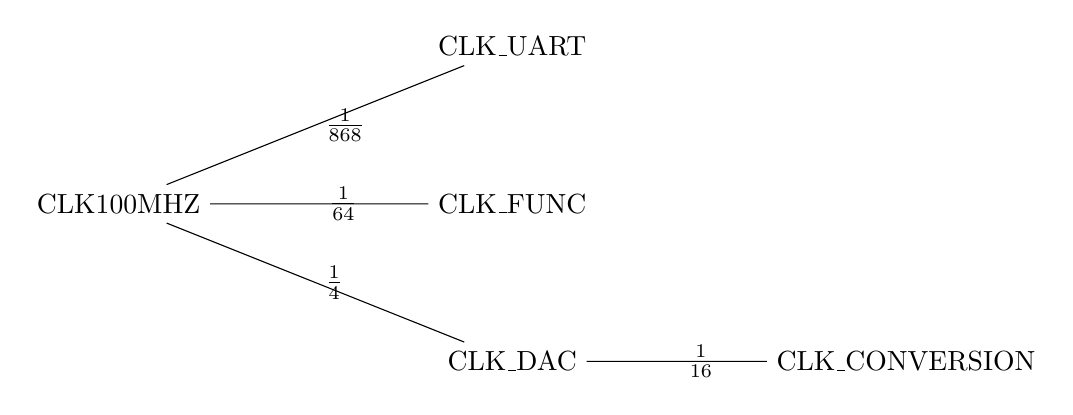
\begin{tikzpicture} 
    \node {CLK100MHZ}[grow=east, sibling distance=2cm, level distance=5cm]
    child {node {CLK\_DAC}
      child {node {CLK\_CONVERSION}
      edge from parent node [right] {$\frac{1}{16}$}}
      edge from parent node [right] {$\frac{1}{4}$}}
    child {node {CLK\_FUNC}
      edge from parent node [right] {$\frac{1}{64}$}}
    child {node {CLK\_UART}
      edge from parent node [right] {$\frac{1}{868}$}};
  \end{tikzpicture} 
  \caption{Clock-Tree} \label{clk:clocktree}
\end{figure}

